% kernel and make the system bootable 

\chapter{ Configuration du noyau et amorçage du système et systemV}
\minitoc
\clearpage

\label{sec:kernel-boot}
\section{Introduction}
Démarrer un système Linux implique plusieurs tâches :  
le processus doit monter les systèmes de fichiers virtuels et réels, initialiser les périphériques, vérifier l’intégrité des systèmes de fichiers, monter et activer les partitions ou fichiers d’échange (swap), régler l’horloge système, mettre en service le réseau, démarrer les démons requis et accomplir toute autre tâche personnalisée spécifiée par l’utilisateur.  

\medskip  
Ce processus doit être organisé pour garantir l’exécution des tâches dans le bon ordre et assurer une rapidité optimale.

\section{Configuration des scripts System V}
\label{sssec:sysv-scripts}

System V est le processus d’amorçage classique sous Linux (cf. chapitre \textcolor{blue}{\ref{sssec:sysv}}). Les scripts suivants sont installés dans \texttt{/etc/rc.d} avec un lien symbolique dans \texttt{/etc/init.d}:



\begin{table}[H]
  \centering
  \caption{Exemple Scripts System V et leurs descriptions}
  \label{tab:sysv-scripts}
  \begin{tabularx}{\linewidth}{|l|X|}
    \toprule
    \textbf{Script} & \textbf{Description} \\
    \midrule
    checkfs      & Vérifie l’intégrité des systèmes de fichiers avant leur montage . \\ \hline
    cleanfs      & Supprime les fichiers temporaires entre redémarrages (\texttt{/run}, \texttt{/var/lock}) . \\ \hline
    console      & Charge la table de clavier appropriée et définit la police d’écran. \\ \hline
    halt         & Arrête et éteint le système. \\ \hline
    ifdown       & Désactive une interface réseau. \\ \hline
    ifup         & Active et configure une interface réseau.  \\ \hline
    mountfs      & Monte tous les systèmes de fichiers . \\ \hline
    mountvirtfs  & Monte les systèmes de fichiers virtuels du noyau (\texttt{proc}, \texttt{sysfs}, \texttt{devpts}, \texttt{run}). \\ \hline
    reboot       & Redémarre le système. \\ \hline
    setclock     & Réinitialise l’horloge système à l’heure locale . \\ \hline
    swap         & Active et désactive les partitions ou fichiers d’échange (\texttt{swap}). \\ \hline
     
    \bottomrule
  \end{tabularx}
\end{table}

Tous ces scripts suivent le même modèle : une structure basée sur une simple  `case statement` qui gère les arguments `start`|`stop`|`restart`.  

\begin{figure}[H]  
  \centering  
  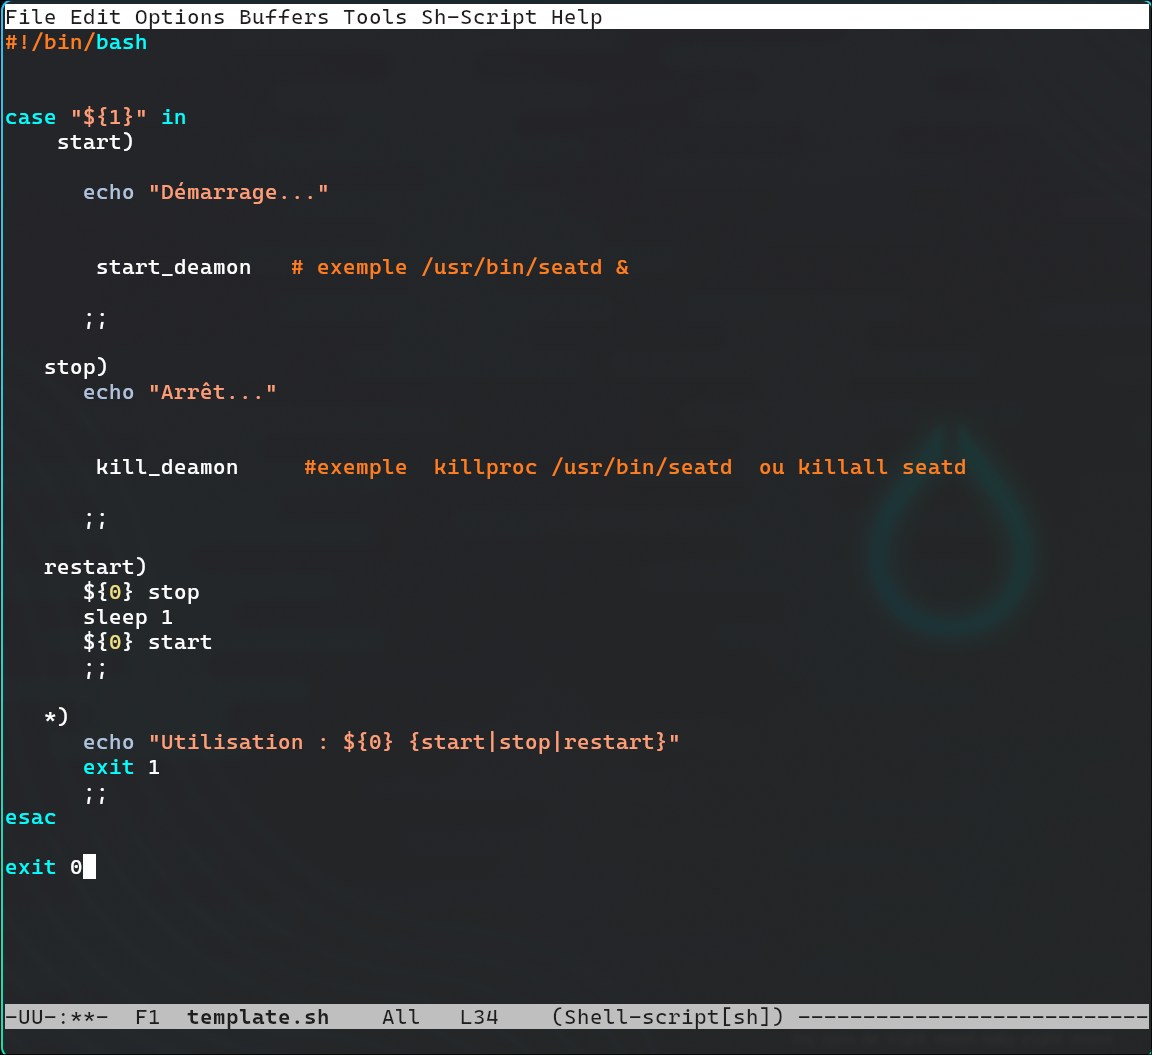
\includegraphics[width=1\textwidth]{images_pfe/systemvtemplate.png}  
  \caption{Exemple de template d’un script de démarrage} 
  \label{fig:systemvtemplate}  
\end{figure}  
\textbf{Remarque} : Nous utilisons les scripts de démarrage de BLFS, que nous avons enrichis avec d'autres simple scripts.  
\textcolor{blue}{Pour plus d'informations sur les scripts BLFS, consultez \cite{blfs_bootscripts}.}

%\subsection{Configurations importantes}
%\label{subsec:config-importantes}

%La configuration du système requiert plusieurs fichiers critiques à ajuster :

%\begin{itemize}
 % \item \textbf{Configuration de l’horloge système} — %\texttt{/etc/sysconfig/clock}  
 % Ce fichier définit le comportement de l’horloge (UTC ou heure locale).
 % simplement ellecentien 
 % \begin{verbatim}
 %     UTC=1 #mean set hardware clock  to UTC (Coordinated Universal Time).
 % \end{verbatim}

  %\item \textbf{Configuration de la console Linux} — %\texttt{/etc/sysconfig/console}  
  %Permet de spécifier la table de caractères, la police et la disposition du %clavier.
  % \begin{verbatim}
  %    LOGLEVEL="3"  # Kernel log verbosity level
  %    UNICODE="1"  # Enable Unicode support
  %    FONT="Lat2-Terminus16". # Console font to use
      
  %\end{verbatim}

  %\item \textbf{Configuration de la locale système} et création de %\texttt{/etc/profile}  
  %Le fichier \texttt{/etc/locale.conf} définit la langue et le jeu de %caractères par défaut 

 

  %\item \textbf{Liste des shells valides} — \texttt{/etc/shells}  
  %Contient les chemins des interpréteurs de commandes autorisés pour les %utilisateurs.

  

  %\item \textbf{Configuration réseau} — %\texttt{/etc/sysconfig/ifconfig.enp0s3}, , \texttt{/etc/hosts}  
  %Ces fichiers déterminent l’adresse IP statique, les serveurs DNS et la %résolution locale des noms d’hôtes.

  
%\end{itemize}

\section{Compilation et paramétrage du noyau Linux}
\label{subsec:compilation-noyau}

Notre implémentation s’appuie sur le noyau version \texttt{6.5.10}, retenu pour son support matériel étendu et ses correctifs de sécurité récents. Nous devons configurer, compiler puis installer ce noyau.

Le noyau Linux comporte environ 12 000 options de configuration. Il est essentiel de sélectionner précisément celles dont nous avons besoin pour optimiser la taille, la sécurité et les performances.
\clearpage
La configuration du noyau Linux s'effectue généralement via l'interface menuconfig, accessible grâce à la commande :\\
\begin{verbatim}
   make menuconfig
\end{verbatim}

\begin{figure}[H]
  \centering
  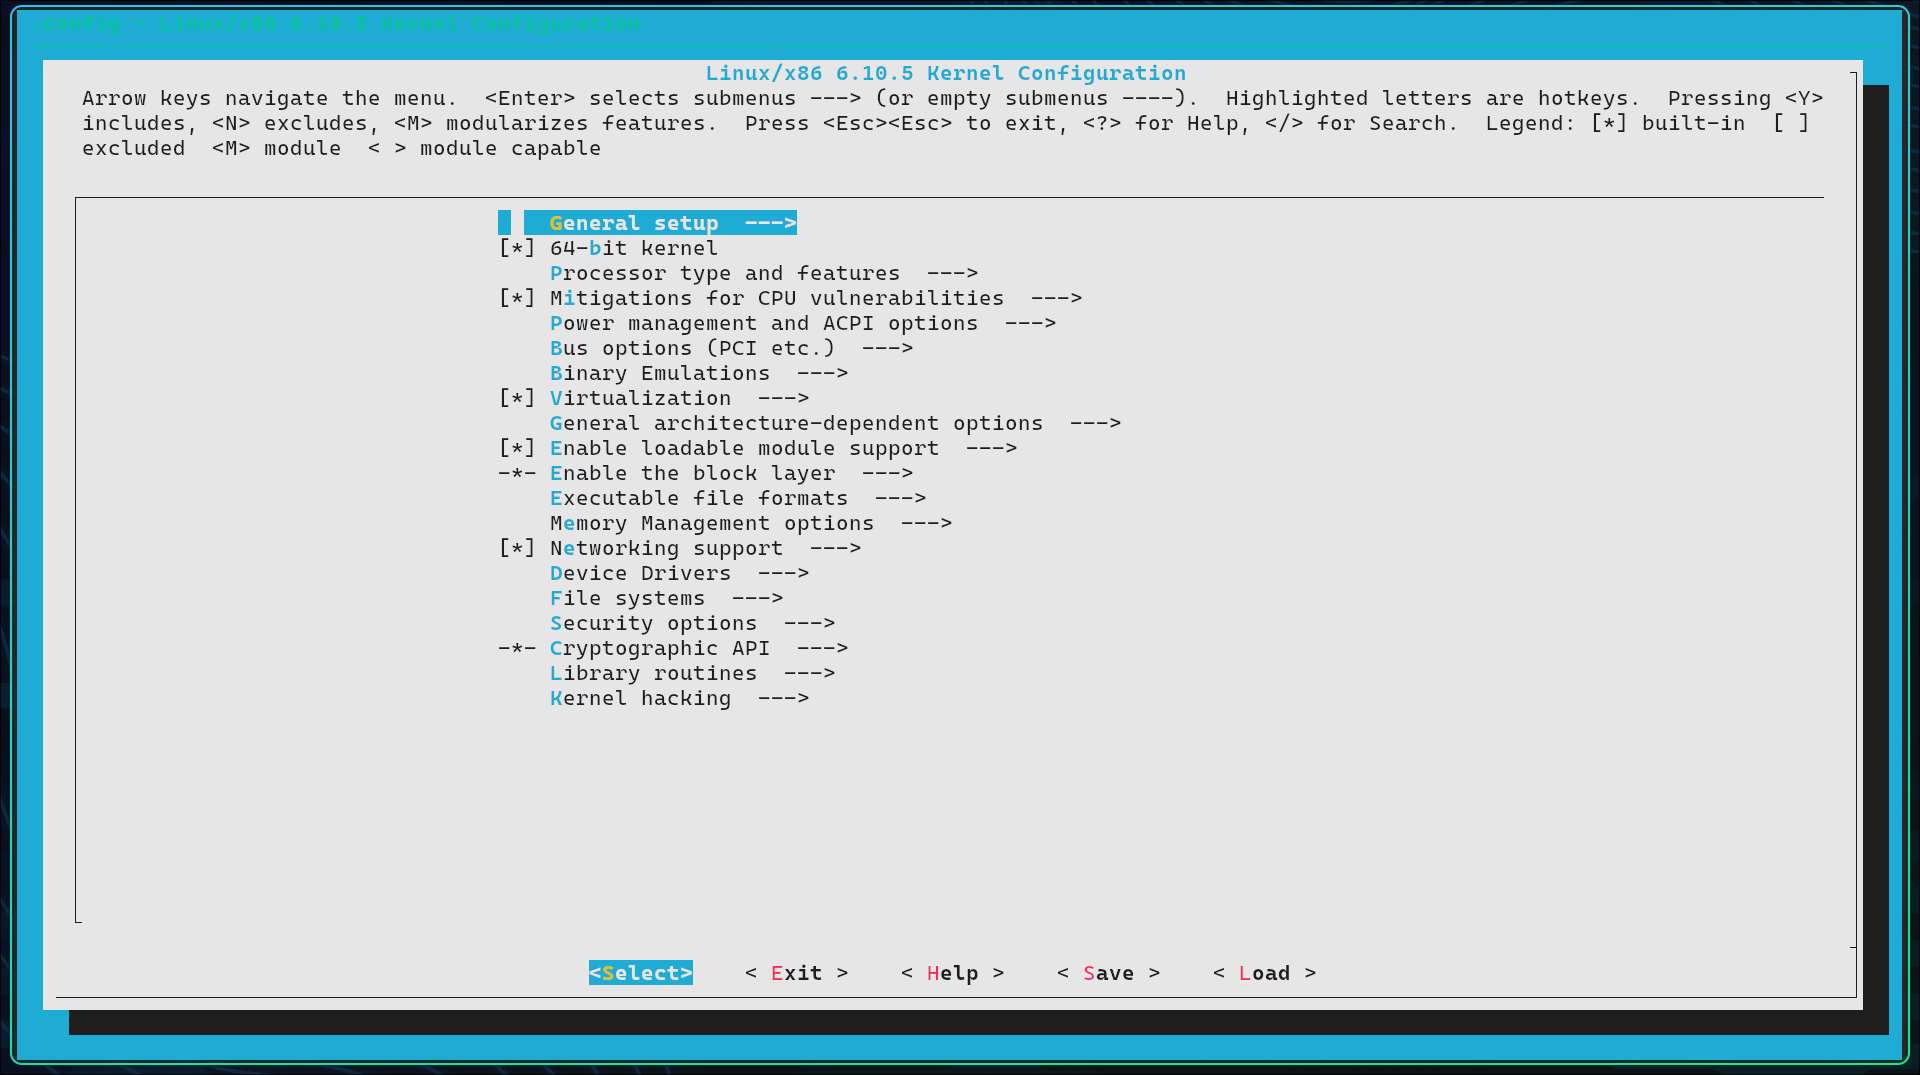
\includegraphics[width=1\textwidth]{images_pfe/kernelmenuconfig.png}
  \caption{Configuration de noyau linux}
  \label{fig:configuration de noyau}
\end{figure}
Nous avons activé environ 1 695 paramètres de configuration.

\textbf{Remarque} : nous n'avons pas configuré manuellement les 1 695 options. Lors de la première étape, nous nous sommes appuyés sur la commande \textbf{make defconfig}, qui génère une configuration de base adaptée à notre architecture \textbf{x86\_64}. 

Ensuite, à l'étape 2, nous avons utilisé \texttt{make menuconfig} pour activer manuellement d'autres options supplémentaires, soit en tant qu’intégrées (\texttt{<*>}), soit en tant que modules (\texttt{<m>}).

Voici un exemple de ces paramètres activés :

\begin{figure}[H]  
  \centering  
  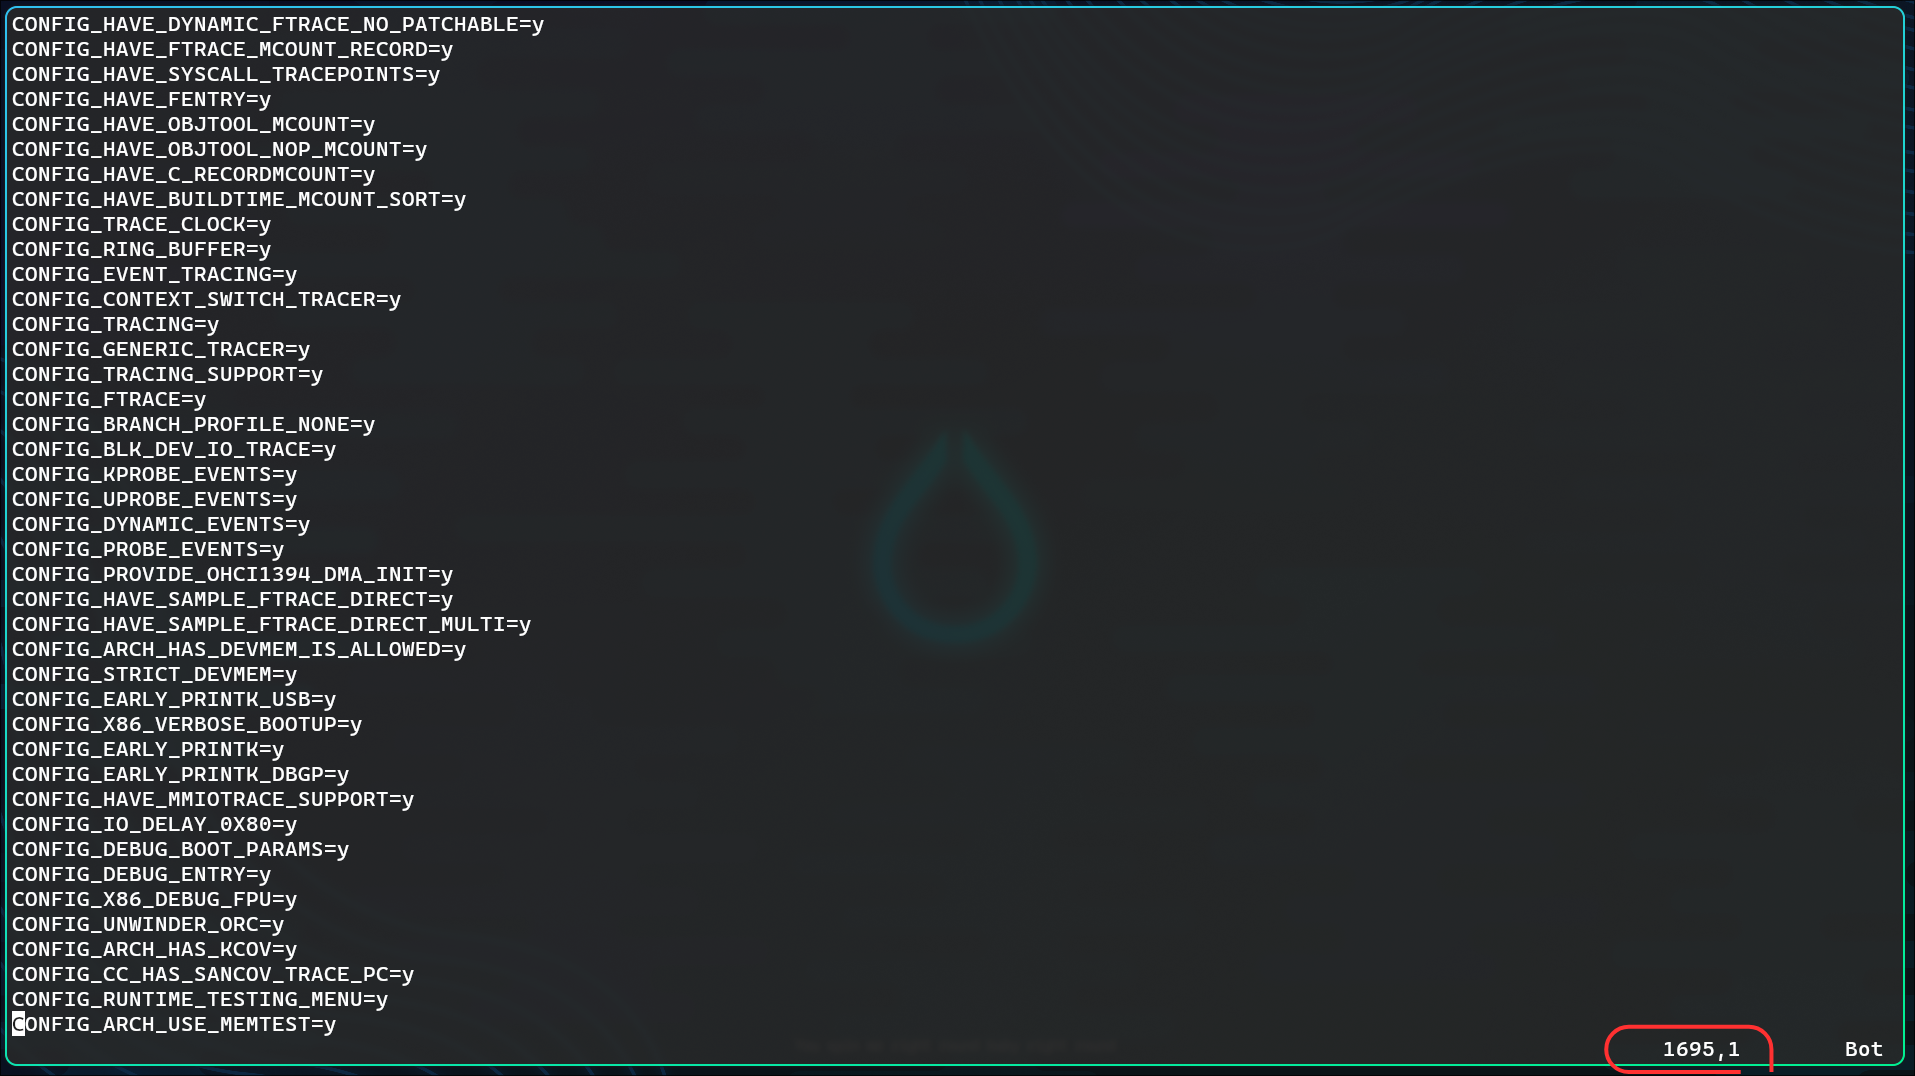
\includegraphics[width=1\textwidth]{images_pfe/numberconfig.png}  
  \caption{Aperçu des paramètres de configuration activés dans \texttt{/boot/config}}  
  \label{fig:kernel_config}  
\end{figure}  



\clearpage
\paragraph*{Fichiers critiques après installation}
\begin{itemize}
  \item \texttt{arch/x86/boot/bzImage} — image binaire du noyau   
  \item \texttt{.config} — fichier de configuration contenant toutes les options sélectionnées  
\end{itemize}

\textit{Remarque :} ces fichiers doivent être configure dans \texttt{/boot} pour être détectés par le chargeur d’amorçage (GRUB) :

\begin{verbatim}
 if faut copier:
 arch/x86/boot/bzImage  dans /boot/vmlinuz-kraken
 config              dans /boot/config
\end{verbatim}


\textcolor{blue}{Pour plus d’informations sur la configuration et la compilation de noyau, consultez \cite{linuxkernel}}
\section{Configuration du processus de démarrage}
\label{sssec:boot}

Le processus de démarrage s’appuie sur deux fichiers principaux : \texttt{/etc/fstab}, qui définit comment et où les périphériques de stockage  sont montés dans la structure de répertoires du système au démarrage, et le fichier de configuration de GRUB \texttt{grub.cfg}.


\begin{enumerate}

  \item \textbf{Exemple de Fichier \texttt{/etc/fstab}}  
  
  \begin{verbatim}


# système de fichiers | point de montage| type | options | dump |fsck-order
#monter les partitions du disque
/dev/sda4      /              ext4     defaults            1     1
/dev/sda3      swap           swap     pri=1               0     0
/dev/sda1      /boot/efi      vfat     codepage=437        0     1
/dev/sda5      /home          ext4     defaults            1     2

#monter les systèmes de fichiers virtuels
proc           /proc          proc     nosuid,noexec,nodev 0     0
sysfs          /sys           sysfs    nosuid,noexec,nodev 0     0
devpts         /dev/pts       devpts   gid=5,mode=620      0     0
tmpfs          /run           tmpfs    defaults            0     0
devtmpfs       /dev           devtmpfs mode=0755,nosuid    0     0
tmpfs          /dev/shm       tmpfs    nosuid,nodev        0     0



  \end{verbatim}
 \textbf{Explications :}
  \begin{itemize}
    \item \textbf{Les quatre premières lignes} servent à monter les partitions du disque dur et activer la swap.
    \item \textbf{Les sept autres lignes} permettent de monter les systèmes de fichiers virtuels.
    \item \textbf{Options :}
    \begin{itemize}
      \item \textbf{dump :} Détermine si une sauvegarde du système de fichiers doit être effectuée (1 = activé, 0 = désactivé). Généralement activé pour les partitions critiques.
      \item \textbf{fsck-order :} Priorité de vérification du système de fichiers au démarrage (0 = aucune, 1 = première priorité, 2 = seconde).\\
    \end{itemize}
  \end{itemize}


  \item \textbf{ Exemple Fichier de configuration de GRUB}  

  \begin{verbatim}

set default=0
set timeout=10
insmod ext2
set root=(hd0,4) 

menuentry "KRAKEN-OS (mode normal)" {
    linux /boot/vmlinuz_kraken root=/dev/sda4 ro
}

menuentry "KRAKEN-OS (mode debug)" {
    linux /boot/vmlinuz_kraken root=/dev/sda4 debug ro
}

menuentry "KRAKEN-OS (mode RAM)" {
    linux /boot/vmlinuz_kraken root=/dev/sda4 ram ro
}

  \end{verbatim}
\end{enumerate}
\textbf{Explications :}
  \begin{itemize}
    \item \textbf{default :} Entrée de menu sélectionnée par défaut (0 = première entrée).
    \item \textbf{timeout :} Délai avant le démarrage automatique (10 secondes).
    \item \textbf{insmod :} Charge un module GRUB nécessaire (ici, le support ext2).
    \item \textbf{menuentry :} Définit une entrée de menu avec des paramètres de démarrage spécifiques.
  \end{itemize}


\clearpage
À ce stade, nous pouvons démarrer le système minimal et visualiser le processus de démarrage.

\begin{figure}[H]
    \centering
    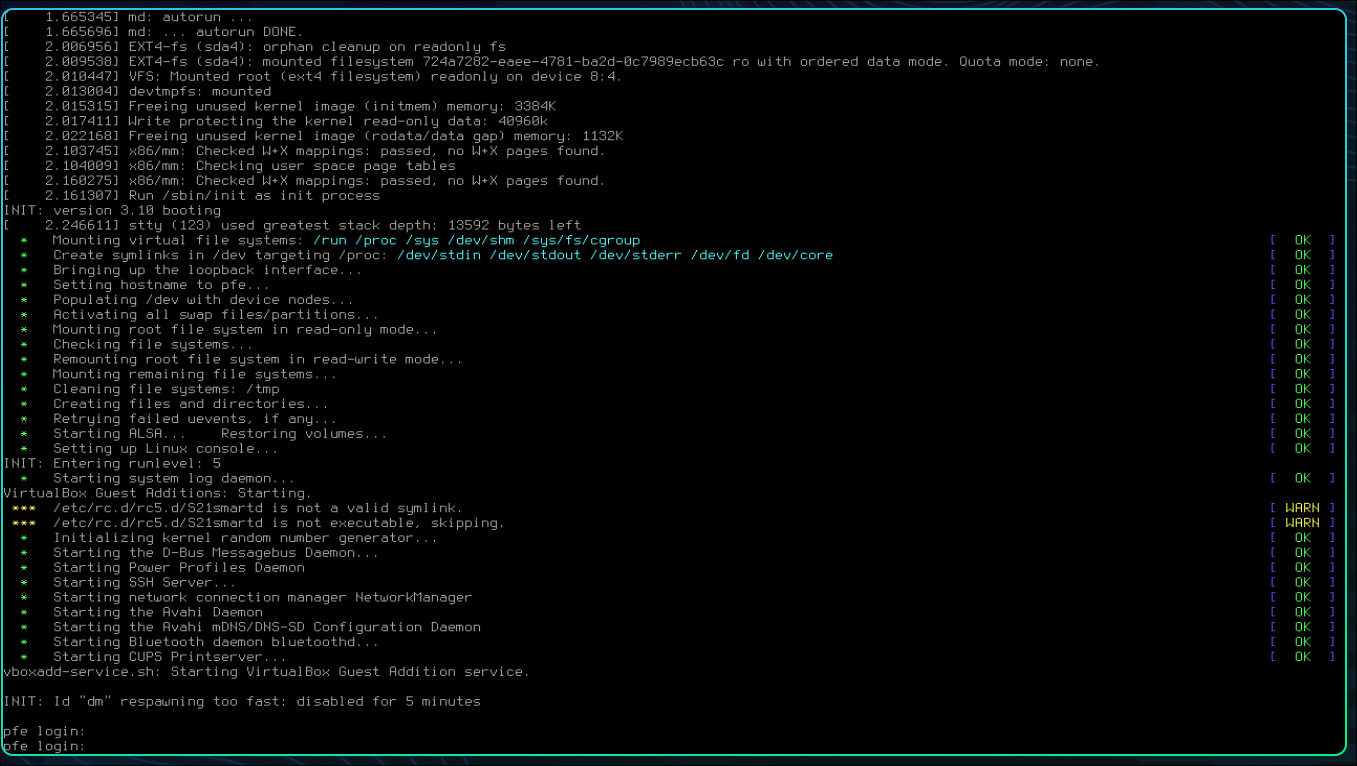
\includegraphics[width=1\textwidth]{images_pfe/corebuildbooscrpts.png}
    \caption{Processus de démarrage}
    \label{fig:bootproc}
\end{figure}

\begin{figure}[H]
    \centering
    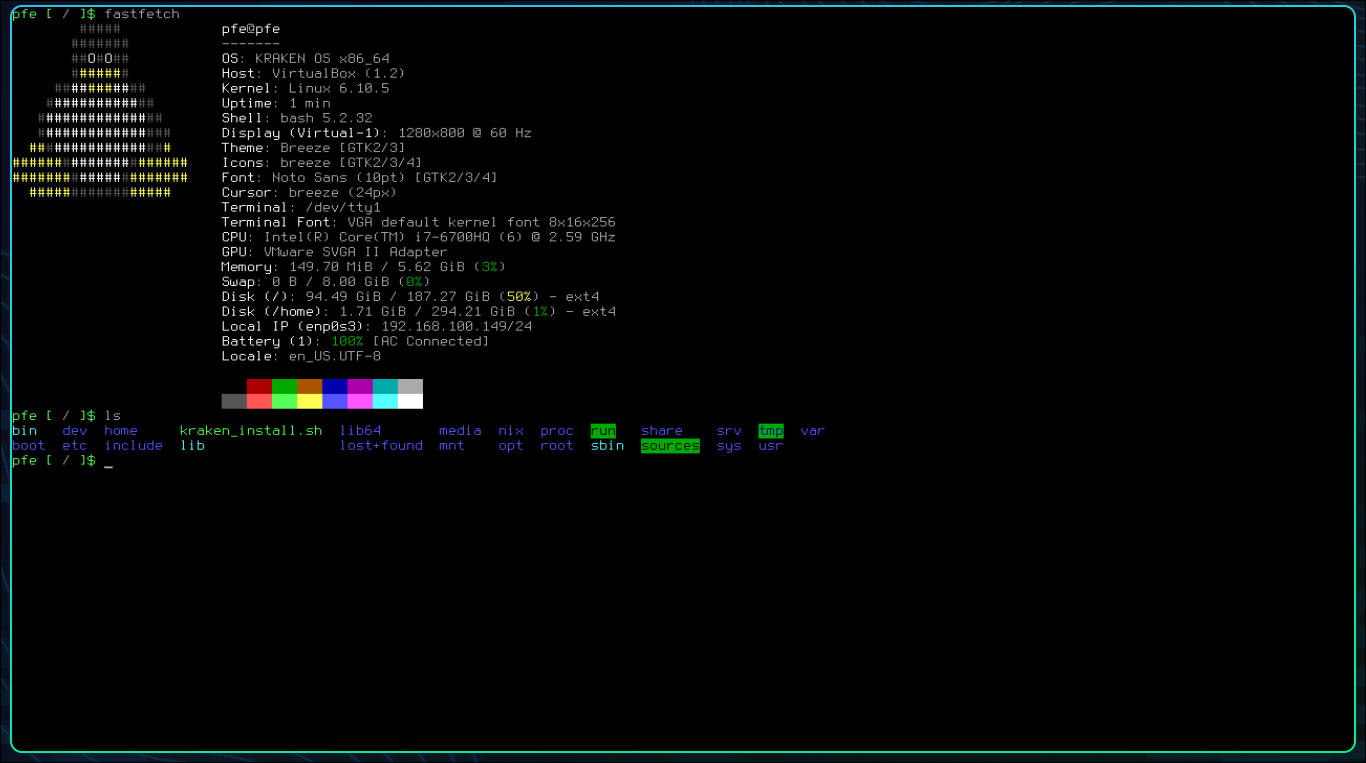
\includegraphics[width=1\textwidth]{images_pfe/corebuildresult.png}
    \caption{Interface TTY du système minimal \textsc{Kraken OS}}
    \label{fig:tty}
\end{figure}

\section{Conclustion}
À ce stade, nous disposons d’une distribution Linux minimale et fonctionnelle, capable de démarrer et d’exécuter des commandes de base.\\
Dans le prochain chapitre, nous passerons à l’étape cruciale : transformer cette base en un système complet et polyvalent.